\section{Results}
\label{sec:results}

\subsection{Facts stated outside English are hard to find again}
\label{sec:main}
Table~\ref{tab:main} gives Recall@5 for English questions by the form in which the facts were stored. For every retriever, moving the same fact out of English costs recall; \NumSigCells{} of the \NumCells{} non-English cells differ significantly from the same retriever's English cell (McNemar, $p<0.01$).

The two non-neural or English-only baselines fail in characteristic ways. BM25 is weak even in English (\RBMHiEn\%), because questions and statements share few words by design, and it finds essentially nothing in any non-English form. The English-only encoder used by default in A-Mem retrieves \RMiniEnHiEn\% of English-stated facts. Its recall drops to \RMiniEnHiMoN\% and \RMiniEnKnMoN\% when the fact is written in native-script Hindi or Kannada, scripts it cannot represent. On native-script \emph{code-mixed} text it retains \RMiniEnHiCmN\% and \RMiniEnKnCmN\%, entirely through the English words embedded in it.

Multilingual encoders fare better but still lose much of their recall. Averaged over the \NumMulti{} multilingual and Indic encoders, Recall@5 falls from \RavgHiEn\% (\form{EN}) to between \RavgHiMoR\% and \RavgHiCmN\% for the Hindi forms, and from \RavgKnEn\% to between \RavgKnMoR\% and \RavgKnCmN\% for the Kannada forms. Kannada is harder than Hindi in every form. The strongest English retriever, mE5-base (\RmEbaseHiEn\%), keeps only \RmEbaseHiCmR\% on Hinglish and \RmEbaseKnCmR\% on Kannada--English, and \RmEbaseHiMoR\% and \RmEbaseKnMoR\% on Romanized monolingual text. BGE-M3 is the most robust to native script, nearly matching its English level on code-mixed native text (\RBGEHiCmN\% and \RBGEKnCmN\% versus \RBGEHiEn\% on \form{EN}). Yet the same words in Latin script fall to \RBGEHiCmR\% and \RBGEKnCmR\%.

The Indic-specialised encoders have the smallest positive gaps (\IndicGapMin--\IndicGapMax{} points), mostly because their English recall is low (\RIndSBHiEn\% and \RVyakHiEn\%). LaBSE, trained for bitext mining, is an outlier. It aligns translations perfectly: for every Hindi fact in our pool, it ranks the English version of the same fact first. But it is poor at matching questions to statements, especially in English. No retriever is both strong on English and robust across forms.

\begin{table}[t]
\centering
\small
\setlength{\tabcolsep}{4pt}
\caption{Recall@5 (\%) of the target memory among 336 pooled memories, for English questions, when the fact was stored in each form (Raw indexing). Each cell averages 240 facts; 95\% bootstrap CIs are about $\pm$6 points. \textbf{Bold}: best retriever per column. $^\dagger$: not significantly different from the same retriever's \form{EN} score (McNemar, $p\ge 0.01$); all other non-EN cells differ significantly.}
\label{tab:main}
\begin{tabular}{@{}l ccccc ccccc@{}}
\toprule
 & \multicolumn{5}{c}{Hindi pool} & \multicolumn{5}{c}{Kannada pool} \\
\cmidrule(lr){2-6}\cmidrule(lr){7-11}
Retriever & EN & CM-R & CM-N & MO-N & MO-R & EN & CM-R & CM-N & MO-N & MO-R \\
\midrule
bm25 & 17.9 & 0.4 & 0.0 & 0.0 & 0.0 & 16.2 & 0.0 & 0.0 & 0.0 & 0.0 \\
MiniLM-en & 64.2 & 23.8 & 37.1 & 0.4 & 6.7 & 63.7 & 32.1 & 42.1 & 0.0 & 9.6 \\
\midrule
mMiniLM & 54.6 & 26.7 & 52.5$^\dagger$ & 50.8$^\dagger$ & 7.9 & 54.6 & \textbf{33.3} & 15.0 & 1.7 & 7.1 \\
mE5-small & 48.8 & \textbf{41.7}$^\dagger$ & 27.1 & 18.8 & 5.8 & 42.5 & 15.4 & 18.3 & 12.1 & 1.7 \\
mE5-base & \textbf{75.4} & 33.3 & 29.2 & 23.3 & 4.6 & \textbf{70.4} & 16.7 & 14.6 & 10.4 & 0.8 \\
LaBSE & 7.9 & 5.8$^\dagger$ & 38.8 & 35.4 & 0.0 & 6.7 & 2.9$^\dagger$ & 25.4 & 39.6 & 0.0 \\
BGE-M3 & 67.9 & 20.4 & \textbf{63.3}$^\dagger$ & \textbf{56.2} & 2.5 & 65.0 & 14.2 & \textbf{60.0}$^\dagger$ & \textbf{51.2} & 1.2 \\
\midrule
IndicSBERT & 37.5 & 25.8 & 29.2 & 34.2$^\dagger$ & \textbf{18.3} & 35.0 & 15.0 & 24.2 & 31.7$^\dagger$ & \textbf{10.0} \\
Vyakyarth & 35.8 & 16.2 & 29.2 & 31.7$^\dagger$ & 4.6 & 35.4 & 12.5 & 29.2$^\dagger$ & 33.3$^\dagger$ & 1.7 \\
\midrule
Avg.\ multilingual & 46.8 & 24.3 & 38.5 & 35.8 & 6.2 & 44.2 & 15.7 & 26.7 & 25.7 & 3.2 \\
\bottomrule
\end{tabular}
\end{table}


\begin{figure}[t]
\centering
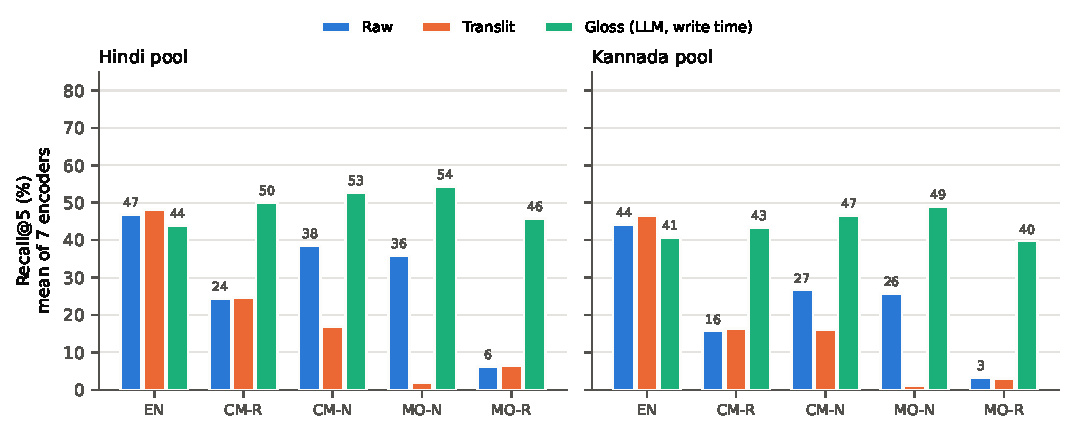
\includegraphics[width=\linewidth]{figures/fig_forms.pdf}
\caption{Recall@5 for English questions by the form in which the fact was stored, averaged over the \NumMulti{} multilingual and Indic encoders. \textbf{Raw}: memories indexed as written. \textbf{Translit}: deterministic script unification. \textbf{Gloss}: an LLM-written English gloss indexed alongside each memory. Labels give Raw and Gloss values; Table~\ref{tab:mitigation} reports per-retriever numbers.}
\label{fig:forms}
\end{figure}

\subsection{Romanization, not code-mixing, drives the loss}
\label{sec:factorial}
The parallel $2\times2$ design separates the two properties that distinguish Indian chat from English (Table~\ref{tab:factorial}).

\paragraph{Code-mixing helps.} Averaged over multilingual encoders, code-mixed memories are retrieved \EffHiMix{} (Hindi) and \EffKnMix{} (Kannada) points \emph{more} often than the same content in monolingual form. The English words that code-mixed users naturally include, such as \emph{shift}, \emph{flat} and \emph{office}, anchor the memory to an English question. The effect is largest for English-centric retrievers: +\MixMiniEnHi{} and +\MixMiniEnKn{} points for the English-only encoder, and +\MixmEbaseHi{} and +\MixmEbaseKn{} for mE5-base.

\paragraph{Romanization hurts.} The same words written in native script are retrieved \EffHiScript{} (Hindi) and \EffKnScript{} (Kannada) points more often than in Latin script, and about \ScriptBGE{} points more often for BGE-M3.

\paragraph{The two effects compound.} Romanized monolingual text, which has neither English anchors nor native script, is the worst condition for nearly every encoder, averaging \RavgHiMoR\% (Hindi) and \RavgKnMoR\% (Kannada). This mirrors the finding of \citet{codemixtax2026} for question answering, and we show it also holds for retrieval in memory. It matters in practice, because Romanized Hindi and Kannada are what many users actually type.

\paragraph{Regression analysis.} A logistic regression on all \NumMulti{}-encoder outcomes, with retriever fixed effects and fact-clustered standard errors (Table~\ref{tab:regression}), confirms the pattern. Among Romanized memories, code-mixing multiplies the odds of retrieval by \ORMix{}. Among monolingual memories, native script multiplies them by \ORNat{}. The negative interaction (odds ratio \ORInt{}) shows that the two aids partly substitute for each other. Kannada lowers the odds by a factor of \ORKan{} relative to Hindi.

\paragraph{Why Romanized text is hard.} Tokenisation offers part of the explanation (Table~\ref{tab:fertility}). The XLM-R tokeniser shared by mE5 and BGE-M3 splits Romanized monolingual words into \FertXHiMoR{} (Hindi) and \FertXKnMoR{} (Kannada) pieces on average. The same words in native script take \FertXHiMoN{} and \FertXKnMoN{} pieces, and English takes \FertXEn{}. Romanized Indic words are thus cut into short, English-looking fragments that carry little of their meaning. The English-only tokeniser maps most Kannada-script tokens to \texttt{[UNK]}, which explains why that encoder cannot retrieve native Kannada at all.

\begin{table}[t]
\centering
\small
\caption{Decomposing the drop (Recall@5 points, English questions, Raw indexing). \emph{Mixing} = mean(CM forms) $-$ mean(MO forms): positive means code-mixed memories are easier to find. \emph{Script} = mean(native forms) $-$ mean(Romanized forms): positive means native script is easier. \emph{EN gap} = EN $-$ mean of the four non-English forms. 95\% bootstrap CIs over facts are given for the average row.}
\label{tab:factorial}
\begin{tabular}{@{}l ccc ccc@{}}
\toprule
 & \multicolumn{3}{c}{Hindi} & \multicolumn{3}{c}{Kannada} \\
\cmidrule(lr){2-4}\cmidrule(lr){5-7}
Retriever & Mixing & Script & EN gap & Mixing & Script & EN gap \\
\midrule
MiniLM-en & +26.9 & +3.5 & +47.2 & +32.3 & +0.2 & +42.8 \\
mMiniLM & +10.2 & +34.4 & +20.1 & +19.8 & -11.9 & +40.3 \\
mE5-small & +22.1 & -0.8 & +25.4 & +10.0 & +6.7 & +30.6 \\
mE5-base & +17.3 & +7.3 & +52.8 & +10.0 & +3.8 & +59.8 \\
LaBSE & +4.6 & +34.2 & -12.1 & -5.6 & +31.0 & -10.3 \\
BGE-M3 & +12.5 & +48.3 & +32.3 & +10.8 & +47.9 & +33.3 \\
IndicSBERT & +1.2 & +9.6 & +10.6 & -1.2 & +15.4 & +14.8 \\
Vyakyarth & +4.6 & +20.0 & +15.4 & +3.3 & +24.2 & +16.2 \\
\midrule
Avg.\ multilingual & +10.4 [9, 12] & +21.8 [20, 24] & +20.7 [19, 23] & +6.7 [5, 8] & +16.7 [15, 19] & +26.4 [24, 28] \\
\bottomrule
\end{tabular}
\end{table}

\begin{table}[t]
\centering
\small
\caption{Logistic regression of Recall@5 success on the properties of the stored form (13,440 retrieval outcomes: 240 facts $\times$ 8 non-English forms $\times$ 7 multilingual and Indic encoders; Raw indexing, English questions). Retriever fixed effects are included; standard errors are clustered by fact. OR: odds ratio with 95\% CI.}
\label{tab:regression}
\begin{tabular}{@{}l c c c c@{}}
\toprule
Term & $\beta$ & SE & OR [95\% CI] & $p$ \\
\midrule
Code-mixed (vs.\ monolingual) & +1.65 & 0.13 & 5.20 [4.04, 6.69] & $<$0.001 \\
Native script (vs.\ Latin) & +2.24 & 0.14 & 9.43 [7.21, 12.33] & $<$0.001 \\
Code-mixed $\times$ native & -1.56 & 0.13 & 0.21 [0.16, 0.27] & $<$0.001 \\
Kannada (vs.\ Hindi) & -0.54 & 0.04 & 0.58 [0.54, 0.63] & $<$0.001 \\
\bottomrule
\end{tabular}
\end{table}

\begin{table}[t]
\centering
\small
\setlength{\tabcolsep}{4pt}
\caption{Tokeniser fertility (subword tokens per whitespace word) of each stored form, averaged over the 240 facts; in parentheses, share of tokens mapped to \texttt{[UNK]}.}
\label{tab:fertility}
\begin{tabular}{@{}l c cccc cccc@{}}
\toprule
 & & \multicolumn{4}{c}{Hindi} & \multicolumn{4}{c}{Kannada} \\
\cmidrule(lr){3-6}\cmidrule(lr){7-10}
Tokeniser & EN & CM-R & CM-N & MO-N & MO-R & CM-R & CM-N & MO-N & MO-R \\
\midrule
XLM-R (mE5, BGE-M3) & 1.3 & 1.5 & 1.3 & 1.5 & 1.7 & 2.0 & 1.8 & 2.3 & 2.8 \\
BERT-en (MiniLM-en) & 1.2 & 1.7 & 2.1 (4\%) & 2.8 (5\%) & 2.1 & 2.1 & 1.3 (47\%) & 1.2 (80\%) & 3.3 \\
\bottomrule
\end{tabular}
\end{table}


\subsection{Questions in the user's language do not rescue retrieval}
\label{sec:reverse}
A code-mixed user may also ask questions in code-mixed form. Figure~\ref{fig:reverse} varies the question form. Matching the question's form to the memory's form helps only partly: with a Romanized code-mixed question over Romanized code-mixed memories, or a native-script question over native-script memories, mean Recall@5 is \SameFormRaw\%, still below the English--English level (\EnAvgRaw\%). Across all non-English question and memory forms, Raw indexing reaches \RevAvgRaw\%. Translating only the question into English (QT) barely helps (\RevAvgQt\%), because the memory remains in the hard form. Adding the write-time gloss (Gloss+QT) raises Recall@5 to \RevAvgGlQt\%.

\begin{figure}[t]
\centering
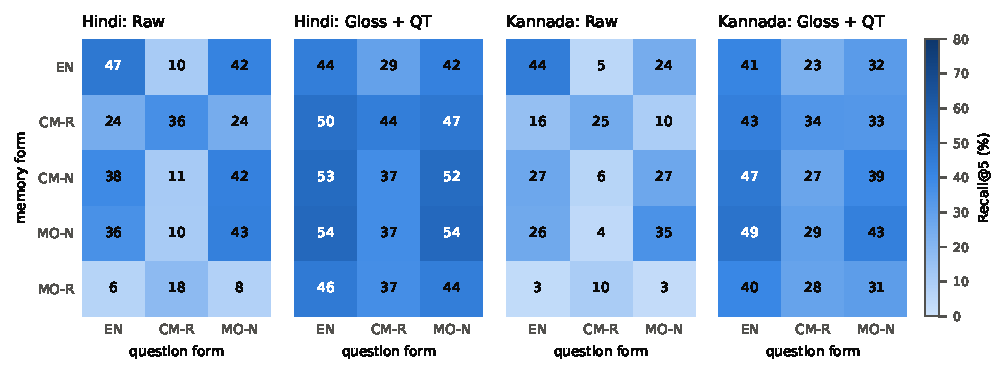
\includegraphics[width=\linewidth]{figures/fig_reverse.pdf}
\caption{Recall@5 by memory form (rows) and question form (columns), averaged over the multilingual and Indic encoders, without mitigation (Raw) and with mitigation (Gloss+QT).}
\label{fig:reverse}
\end{figure}

\subsection{Mitigations: unify the script, or write an English gloss}
\label{sec:mitigation}
Table~\ref{tab:mitigation} compares the mitigations for English questions.

\paragraph{Script unification backfires.} Deterministically romanizing every native-script memory and question lowers mean non-English Recall@5 from \MitAvgRaw\% to \MitAvgTranslit\%. It converts the comparatively easy native-script forms into the hardest one, Romanized text. Converting in the other direction would require resolving the ambiguity of casual Romanized spelling, a learned transliteration problem \citep{madhani2023aksharantar}, and would still leave the English words of code-mixed text in a script the encoder represents poorly.

\paragraph{An English gloss at write time closes most of the gap.} Indexing an LLM-written English gloss next to each non-English memory raises mean non-English Recall@5 from \MitAvgRaw\% to \MitAvgGloss\% (Hindi \MitAvgRawHi\%\,$\rightarrow$\,\MitAvgGlossHi\%, Kannada \MitAvgRawKn\%\,$\rightarrow$\,\MitAvgGlossKn\%). Every retriever improves on average, as do \NumCellsImproved{} of the \NumCells{} retriever--form cells. The gain is largest where Raw indexing fails most: Romanized monolingual text (+\GainMoR{} points on average) and English-centric encoders (+\GainmEbase{} for mE5-base, +\GainMiniEn{} for the English-only encoder). For every encoder with reasonable English recall, non-English recall under Gloss comes within a few points of its English recall under the same indexing. Where the gloss preserved the answer string, Recall@5 is \GlossKeptRfive\%; where it lost the answer, Recall@5 is \GlossLostRfive\%. Better translation should therefore help further.

\paragraph{Costs of the gloss.} The gloss has two costs. First, English-stated facts can lose a little. The other users' facts and the IndicTalk turns gain English glosses and so compete more strongly with English facts; for mE5-base, English-stated facts fall from \RmEbaseHiEn\% to \GlossEnmEbaseHi\% in the Hindi pool. Second, the gloss needs one extra LLM call per non-English memory. The call is short (a chat message in, one sentence out) and is paid once at write time rather than on every read.

\begin{table}[t]
\centering
\small
\caption{Mitigations, English questions. Mean Recall@5 (\%) over the eight non-English forms (four per language), and the gap to the same retriever's \form{EN} score (averaged over the two pools). Translit: deterministic script unification. Gloss: LLM English gloss indexed next to each memory at write time.}
\label{tab:mitigation}
\begin{tabular}{@{}l c cc cc cc@{}}
\toprule
Retriever & \form{EN} & \multicolumn{2}{c}{Raw} & \multicolumn{2}{c}{Translit} & \multicolumn{2}{c}{Gloss} \\
 & & non-EN & gap & non-EN & gap & non-EN & gap \\
\midrule
bm25 & 17.1 & 0.1 & -17.0 & 0.1 & -17.0 & 16.2 & -1.7 \\
MiniLM-en & 64.0 & 19.0 & -45.0 & 16.5 & -47.4 & 61.8 & +1.0 \\
mMiniLM & 54.6 & 24.4 & -30.2 & 16.8 & -39.5 & 54.5 & +3.1 \\
mE5-small & 45.6 & 17.6 & -28.0 & 11.7 & -31.4 & 44.6 & +1.5 \\
mE5-base & 72.9 & 16.6 & -56.3 & 9.9 & -63.0 & 66.5 & -2.5 \\
LaBSE & 7.3 & 18.5 & +11.2 & 3.3 & -13.2 & 22.8 & +16.8 \\
BGE-M3 & 66.5 & 33.6 & -32.8 & 10.4 & -59.0 & 65.6 & +2.9 \\
IndicSBERT & 36.2 & 23.5 & -12.7 & 15.7 & -20.4 & 39.8 & +7.6 \\
Vyakyarth & 35.6 & 19.8 & -15.8 & 7.7 & -29.6 & 39.9 & +8.3 \\
\bottomrule
\end{tabular}
\end{table}


\subsection{Larger memories}
\label{sec:poolsize}
Real histories hold more than 336 messages. Figure~\ref{fig:poolsize} repeats the main comparison with \PoolNSmall{}, \PoolNDefault{} and about \PoolNLarge{} memories per user; the largest pool uses every admissible distractor in the banks. Absolute recall falls as memories grow, but the ordering is stable, and the relative loss under Raw indexing widens. Non-English recall is 60\% of English recall with \PoolNSmall{} memories and 38\% with about \PoolNLarge{}, while under Gloss it matches or exceeds English recall at every size. With about \PoolNLarge{} memories, English-stated facts reach \PoolLargeRawEN\%, non-English facts \PoolLargeRawnonEN\% under Raw indexing, and \PoolLargeGlossnonEN\% under Gloss.

\begin{figure}[t]
\centering
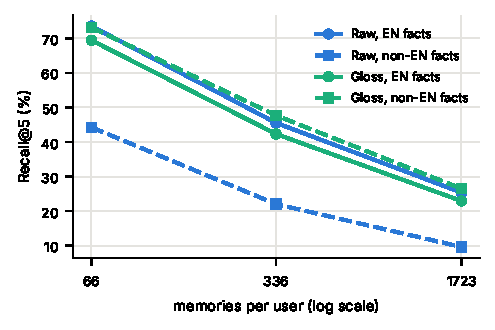
\includegraphics[width=0.46\linewidth]{figures/fig_poolsize.pdf}
\caption{Recall@5 for English questions as the number of memories per user grows, averaged over the \NumMulti{} multilingual and Indic encoders. Colour: indexing (Raw or Gloss). Line style: facts stored in English (solid) or in the eight Hindi and Kannada forms (dashed).}
\label{fig:poolsize}
\end{figure}

\subsection{Retrieval, not reading, is the bottleneck}
\label{sec:e2e}
Table~\ref{tab:e2e} shows what happens when an LLM reader answers from five memories. When the target memory is among them (Oracle), Claude Haiku 4.5 answers \EtoEOracleNonEn\% of non-English and \EtoEOracleEn\% of English facts correctly; it reads Hinglish, Kannada--English and native-script memories about as well as English ones. With mE5-base's top 5 under Raw indexing, accuracy on non-English facts collapses to \EtoERawNonEn\% (English: \EtoERawEn\%), closely tracking how often the target was retrieved. With the gloss in the index it rises to \EtoEGlossNonEn\%, close to the English level under the same indexing (\EtoEGlossEn\%). Across conditions, accuracy is bounded by retrieval: the language barrier in agent memory sits at the retriever, not the LLM.

\begin{table}[t]
\centering
\small
\caption{End-to-end answer accuracy (\%) of an LLM reader (Claude Haiku 4.5) given five memories, for 48 facts (two per relation) and English questions. Raw/Gloss: top-5 memories retrieved by mE5-base under Raw or Gloss indexing; in parentheses, how often the target memory was among them. Oracle: target memory plus four random pool memories.}
\label{tab:e2e}
\begin{tabular}{@{}l ccc@{}}
\toprule
Stored form & Raw & Gloss & Oracle \\
\midrule
\form{EN} & 72.9 (75) & 66.7 (69) & 95.8 \\
\midrule
\form{hi-CM-R} & 35.4 (35) & 66.7 (71) & 100.0 \\
\form{hi-CM-N} & 25.0 (27) & 66.7 (71) & 97.9 \\
\form{hi-MO-N} & 25.0 (23) & 70.8 (71) & 100.0 \\
\form{hi-MO-R} & 2.1 (2) & 62.5 (62) & 100.0 \\
\midrule
\form{kn-CM-R} & 18.8 (19) & 64.6 (67) & 97.9 \\
\form{kn-CM-N} & 12.5 (12) & 64.6 (69) & 97.9 \\
\form{kn-MO-N} & 10.4 (10) & 58.3 (65) & 97.9 \\
\form{kn-MO-R} & 2.1 (2) & 52.1 (65) & 87.5 \\
\midrule
non-EN mean & 16.4 & 63.3 & 97.4 \\
\bottomrule
\end{tabular}
\end{table}


\section{Discussion}
\label{sec:discussion}

\paragraph{Implications for memory systems.}
Today's defaults fit poorly with how many people actually write. Storing memories in the user's own language and script, as Mem0's input-language mode does \citep{mem0repo}, preserves fidelity. But a store indexed only by that text inherits every weakness of its encoder on Romanized and code-mixed input. An English-only default encoder, as in A-Mem \citep{amemrepo}, cannot represent Devanagari or Kannada at all. Our results support a simple pattern: keep the original text for the reader, and index it together with a canonical English gloss written once at write time. Deterministic script unification is attractive because it needs no model, but it moves memories toward the representation encoders handle worst.

\paragraph{Implications for evaluation.}
Memory benchmarks report a single English number. The gap we measure is far larger than the differences that typically separate memory systems on English benchmarks, so a system's ranking on LoCoMo or LongMemEval says little about how it serves a user who writes ``\emph{yaar finally Pune shift ho gayi}''. Because \lipi{} is parallel and pool-controlled, it can be added to a memory system's evaluation at low cost: its 1{,}920 non-English memories and 1{,}200 questions fit in a single evaluation run.

\paragraph{Toward Romanization-robust encoders.}
Multilingual encoders see Hindi and Kannada mostly in native script during pre-training, and their tokenisers fragment Romanized Indic words. Code-mixed text survives partly because of its English words, while monolingual Romanized text has no such anchor. Romanization-aware pre-training \citep{husain2024romansetu} or contrastive fine-tuning on Romanized and code-mixed pairs are natural next steps. \lipi{}'s parallel forms provide such pairs, though at present only enough for evaluation.

\paragraph{Limitations.}
\begin{itemize}
\item \textbf{Synthetic data.} The facts are LLM-drafted and checked automatically and by an LLM reviewer, not yet by native speakers. Real chat is noisier: inconsistent spellings, typos and script switches within a sentence. This plausibly makes our estimates of the problem optimistic.
\item \textbf{One model family.} The drafting, gloss and reader models all come from the Claude family. This could make glosses of Claude-drafted text unusually accurate, so the gloss results should be confirmed with other models.
\item \textbf{Two languages.} We cover two languages, one Indo-Aryan and one Dravidian. Other scripts and code-mixing registers, such as Tamil--English, Bengali--English or Arabizi, may behave differently.
\item \textbf{Simple memories.} Memories are single utterances, and every question targets a single fact. Multi-hop, temporal and knowledge-update questions, where cross-lingual matching interacts with reasoning, are not tested.
\item \textbf{Components, not frameworks.} We evaluate retrieval components and a gloss strategy rather than complete memory frameworks, whose fact-extraction step could itself translate, or garble, code-mixed input.
\item \textbf{Retrievers not evaluated.} Compute limits kept us from evaluating API embedders (such as Mem0's default, \texttt{text-embedding-3-small}) and LLM-based embedders (such as Qwen3-Embedding).
\end{itemize}

\section{Conclusion}
\label{sec:conclusion}
We asked whether an LLM agent's memory still works when a user states a fact in Hinglish, Kannada--English or native-script Hindi or Kannada, and later asks about it in English. Using \lipi{}, a parallel and pool-controlled benchmark, we find that it largely does not. Retrieval loses most of its recall, Romanized monolingual text is nearly unretrievable, and the culprit is romanization rather than code-mixing. Because LLM readers understand these memories once they see them, the fix belongs at indexing time. An English gloss written alongside each non-English memory closes most of the gap, whereas deterministic script unification makes things worse. We release \lipi{} and all model outputs to make language and script robustness a standard part of evaluating agent memory.

\section*{Broader Impact Statement}
Personal assistants that remember are being deployed to users who write in code-mixed and Romanized registers. Our results show that such users silently receive a worse memory, and that an English-only evaluation will not reveal it. Making the gap measurable, and showing an inexpensive way to close it, should help these users; we see no direct path from this work to harm. All users and facts in \lipi{} are fictional. The released distractor corpora are synthetic, CC-BY-4.0 conversations. Glossing memories with an LLM means sending user messages to a model, which deployed systems should handle under the same privacy terms as the memories themselves.

\section*{Reproducibility Statement}
\CodeAvailability{} The benchmark, every per-fact rank, all 5{,}254 glosses and translations, and all reader answers are included, so every table and figure can be regenerated with \texttt{src/analyze.py} and \texttt{src/figures.py} without any API access. The prompts used for drafting, glossing, translating and reading are given in Appendices~\ref{app:style} and~\ref{app:prompts}.
